\chapter{Observations, Curvature, and the Cosmological Fit}

This lecture begins with a refusal to separate observation from dynamics. We are not going to list astronomical facts and only afterward decide what they mean. We are first going to restore the Friedmann equation, the Hubble function, and the geometry of FRW space, and only then ask what astronomers can actually measure. From there the lecture proceeds in a very deliberate sequence: what enters the equation today, how the older open-universe picture arose, why dark matter was the first major correction, and finally how luminosity and number counts as functions of redshift are turned into a fit for the modern values of \(\Omega_m\), \(\Omega_\Lambda\), and \(\Omega_k\). These notes follow Leonard Susskind's lecture closely, with lecture-board evidence preserved from LazyingArt LLC and Video2Book where it materially helps fix equations, diagrams, or board logic.

\section{Friedmann Equation, Hubble Function, and FRW Geometry}

The opening claim is methodological. Observational cosmology only makes sense when observations are tied back to the fundamental equations. So the lecture begins, once again, with the basic equation for a homogeneous universe:
\begin{equation}
\left(\frac{\dot a(t)}{a(t)}\right)^2
=
\frac{8\pi G}{3}\rho(t)-\frac{k}{a(t)^2}.
\end{equation}
Susskind immediately names
\begin{equation}
H(t)=\frac{\dot a(t)}{a(t)}
\end{equation}
the Hubble function. One may call its present value the Hubble constant, but the point of the lecture is that \(H\) is really a function of time, and the distinction matters once we begin looking deep into the past.

The curvature parameter is normalized once and for all:
\begin{equation}
k\in\{+1,0,-1\}.
\end{equation}
These are not merely signs. They label the three spatial geometries: spherical, flat, and hyperbolic.

The role of the scale factor \(a(t)\) is to enter the metric. The lecture compresses the three possible angular factors into a single function \(\xi(r)\), and that is the notation we will keep:
\begin{equation}
ds^2=-dt^2+a(t)^2\left[dr^2+\xi(r)^2\,d\Omega_2^2\right],
\end{equation}
with
\begin{equation}
\xi(r)=
\begin{cases}
\sin r, & k=+1,\\[4pt]
r, & k=0,\\[4pt]
\sinh r, & k=-1.
\end{cases}
\end{equation}
This choice of notation is more than cosmetic. The same \(\xi(r)\) that describes the angular part of the metric will later reappear in the area of spheres, the growth of shell volumes, and therefore in the observable count of galaxies as a function of redshift.

So the stage is now fixed. We have three possible geometries and one equation of motion for \(a(t)\). The rest of the lecture asks what the sky has to say about which choice is right.

\section{What Enters the Equation Today, and What Astronomers Can Measure}

The lecture next turns from geometry to bookkeeping. What, today, sits on the right-hand side of the Friedmann equation? Radiation, matter, vacuum energy, and curvature. In the lecture these are grouped operationally as
\begin{equation}
\frac{C_r}{a^4}+\frac{C_m}{a^3}+\Lambda-\frac{k}{a^2}=H^2.
\end{equation}
Here \(C_r\) and \(C_m\) are constants. Radiation scales as \(a^{-4}\), nonrelativistic matter as \(a^{-3}\), vacuum energy does not dilute, and the curvature term scales as \(a^{-2}\). Strictly speaking curvature is not an energy density, but the lecture momentarily treats it as a fourth contribution in the present-day budget, and that bookkeeping is exactly what motivates the observational discussion.

\begin{definition}
The present-day density parameters are the fractions of \(H_0^2\) carried by each of these terms at the present time:
\begin{equation}
\Omega_r+\Omega_m+\Omega_\Lambda+\Omega_k=1.
\end{equation}
With our sign convention,
\begin{equation}
\Omega_k=\frac{-k/a_0^2}{H_0^2},
\end{equation}
so \(\Omega_k\) can be positive, negative, or zero even though \(k\) itself takes only the values \(+1,0,-1\).
\end{definition}

This is the point at which the lecture asks the practical question: once the four pieces are written, how do we measure any of them?

The first and easiest foothold is \(H_0\). Hubble measured it by relating redshift to distance. Velocity came from redshift; distance came from brightness. The lecture is careful to note that Hubble's original observations were not deep cosmological measurements in the modern sense. They were local enough that he was effectively measuring the present value of the Hubble function, not mapping its time dependence across cosmic history.

Radiation is easier still. The present-day radiation energy density is dominated by the cosmic microwave background, and it is tiny. One does not need a very deep model to know that \(\Omega_r\) is negligible today.

Then comes ordinary visible matter. One looks at galaxies, hydrogen, stellar populations, interstellar gas, and the average properties of stars. The luminous matter can be estimated by techniques that are technical, but not conceptually mysterious. Susskind quotes the present cosmic average very roughly as about one proton per cubic meter.

The lecture now has its present-day budget in hand: \(H_0\) is measurable, radiation is tiny, luminous matter is small but not negligible, and vacuum energy has been deliberately set aside for the moment because the lecture wants to reconstruct the older picture first.

\subsection{Question \& Answer}

A natural objection is raised almost immediately: how can brightness be used as a distance measure at all, unless we already know the intrinsic brightness of what we are looking at?

The answer is the cosmic distance ladder. We do not begin with distant supernovae and guess their luminosities. We begin with the nearest stars, whose distances can be determined by parallax. Among those nearby stars we identify Cepheid variables, whose periods determine their luminosities. That gives us a standard candle which can then be carried outward. Farther up the ladder, supernovae become the best standard candles for the cosmological redshifts of interest.

So distance is not inferred from raw brightness in a single leap. It is inferred from brightness only after a chain of overlapping calibrations has been built. This is why the lecture spends time on the ladder before returning to cosmological fitting: brightness must first be made trustworthy as data.

\section{The Older Cosmological Picture and Why It Seemed to Favor an Open Universe}

Now the lecture becomes explicitly historical. We are to think the way cosmologists once thought, before dark matter had been folded into the matter budget and before \(\Lambda\) returned as a serious cosmological term. In that older picture,
\begin{equation}
\Omega_r\approx 0,\qquad \Omega_\Lambda=0,
\end{equation}
and the matter fraction inferred from luminous matter alone was small:
\begin{equation}
\Omega_m\sim \frac{1}{20}\text{--}\frac{1}{30}.
\end{equation}
Then the sum rule forced
\begin{equation}
\Omega_k\approx 1.
\end{equation}

\begin{figure}
\centering

\includegraphics[width=0.72\textwidth]{lecture_06_figure_02.png}
\caption{Board review of the matter-era scaling law relating \(a(t)\) and the Hubble scale. The frame is cropped, so the legible board remnants are supplemented by a clean reconstruction in the text.}
\end{figure}

At this point the lecture returns to a matter-dominated universe and works out the relation between the Hubble scale and the age of the universe. The matter-dominated solution is
\begin{equation}
a(t)\propto t^{2/3}.
\end{equation}
Differentiating,
\begin{equation}
\dot a(t)\propto \frac{2}{3}t^{-1/3},
\end{equation}
and dividing by \(a(t)\propto t^{2/3}\), we find
\begin{equation}
\frac{\dot a}{a}=\frac{2}{3t}.
\end{equation}
So
\begin{equation}
H(t)=\frac{2}{3t},
\end{equation}
and therefore, evaluated at the present age \(T\),
\begin{equation}
H_0=\frac{2}{3T}.
\end{equation}
This is why the lecture keeps saying that the Hubble constant is, from the theoretical point of view, essentially the inverse age of the universe.

The lecture briefly compares this with the radiation-dominated case,
\begin{equation}
a(t)\propto t^{1/2},
\qquad
H(t)=\frac{1}{2t},
\end{equation}
not because radiation domination is the main case here, but because it reinforces the broader point that for simple equations of state the Hubble scale tracks inverse cosmic age.

A subtlety then appears, and the lecture pauses to address it because a student notices the tension. If curvature was thought to dominate \emph{today}, why are we allowed to use the matter-dominated solution \(a\sim t^{2/3}\)? The answer is that for most of the history of the universe, at smaller \(a\), the matter term \(a^{-3}\) beats the curvature term \(a^{-2}\). Curvature wins only late. So the matter-dominated solution is still a good approximation over most of the past history, and that is enough to make \(H_0\) of order \(1/T\).

Now combine that with the old observational bookkeeping. The luminous matter term was much too small to account for the measured \(H_0^2\). Therefore the remaining contribution had to come from curvature:
\begin{equation}
-\frac{k}{a_0^2}\sim H_0^2.
\end{equation}
Since this term had to be positive, the sign was immediately fixed:
\begin{equation}
k<0.
\end{equation}
So the older inference was an open, negatively curved universe.

If in addition
\begin{equation}
\frac{1}{a_0^2}\sim H_0^2
\end{equation}
and
\begin{equation}
H_0\sim \frac{1}{T},
\end{equation}
then one is driven to the old conclusion that the radius of curvature is of order the age of the universe. In units with \(c=1\), this is a direct comparison of length and time; in ordinary units it means a curvature scale of order \(cT\).

The lecture is emphatic that this is not the modern conclusion. But it is the correct reconstruction of why the old conclusion once seemed natural.

\section{Dark Matter as the First Correction: Rotation Curves and Galactic Halos}

The next major turn is dark matter. Susskind does not introduce it as a slogan but as a discrepancy between luminous matter and gravitating matter. There is matter we know by direct radiation, and there is matter inferred from the way galaxies and clusters of galaxies move. Oort and then Zwicky noticed that the gravitational behavior of galaxies and clusters did not fit the amount of luminous matter that had been counted.

Before the lecture gets to the main derivation, it disposes of a possible red herring. Supermassive black holes at galactic centers are not the missing mass. They are too small a fraction of the total galactic mass, and in any case they are too centrally concentrated. Whatever dark matter is, it is not sitting only at the center.

\begin{figure}
\centering

\includegraphics[width=0.78\textwidth]{lecture_06_figure_03.png}
\caption{Board evidence for the Newtonian force-balance setup used in the rotation-curve argument. Only the numerator \(MG\) and the fraction bar are clearly legible; the completed equation is reconstructed from the lecture's argument.}
\end{figure}

The lecture then slows down and goes through the standard Newtonian logic. Take a galaxy, look at stars at different radii, and measure their tangential velocity \(v\). If all the gravitating matter were concentrated near the center, then an outer star would move in an approximately central field. The transcript is badly garbled at one point here, so we write the canonical equation in cleaned form:
\begin{equation}
\frac{GM}{r^2}=\frac{v^2}{r}.
\end{equation}
Multiplying by \(r\), we obtain
\begin{equation}
v^2=\frac{GM}{r},
\end{equation}
and hence
\begin{equation}
v(r)\propto r^{-1/2}.
\end{equation}
This is simply the Kepler-law falloff.

\begin{figure}
\centering
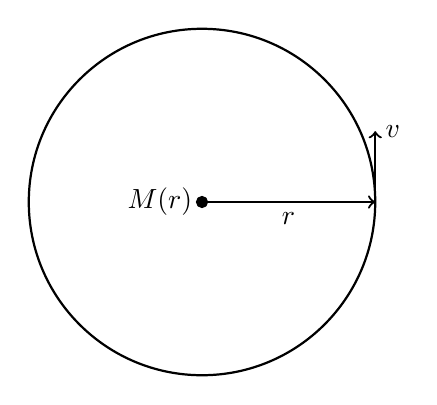
\begin{tikzpicture}[scale=1.0]
\draw[thick] (0,0) circle (2.2);
\filldraw (0,0) circle (2pt);
\draw[->,thick] (0,0)--(2.2,0) node[midway,below] {$r$};
\draw[->,thick] (2.2,0)--(2.2,0.9) node[right] {$v$};
\node[left] at (0,0) {$M(r)$};
\end{tikzpicture}
\caption{Clean reconstruction of the orbit sketch behind the rotation-curve discussion. The central label is written as \(M(r)\) to anticipate the enclosed-mass generalization.}
\end{figure}

But galaxies do not behave that way. Their rotation curves are approximately flat. So we must replace the central mass \(M\) by the enclosed mass \(M(r)\), the total mass inside radius \(r\). Then
\begin{equation}
\frac{G\,M(r)}{r^2}=\frac{v^2}{r}.
\end{equation}
If \(v(r)\) is approximately constant, then
\begin{equation}
M(r)\propto r.
\end{equation}
This is the decisive conclusion. The total mass inside radius \(r\) keeps growing as we move outward. The luminous matter is concentrated toward the center, but the gravitating matter is not.

The lecture is careful to say that this is a statement about enclosed mass, not directly about the local mass density. It is also careful to say that the observed flatness of the rotation curve is itself not explained by a simple elementary argument. It looks neat, almost too neat, and the lecture does not pretend to know a short derivation of why galaxy formation should naturally produce such a profile. What is certain is the observational inference.

There is more. The mass distribution inferred from stellar motions perpendicular to the galactic plane looks roughly spherical, not disk-like. So the picture is not a thin dark disk shadowing the luminous galaxy. It is a large dark halo.

\subsection{Question \& Answer}

At exactly this point the lecture raises the right question: if the dark matter is there, why did it not collapse into the same structure as the luminous matter?

The answer is dynamical. Ordinary luminous matter is made of electrically charged particles. It radiates when accelerated, it collides electromagnetically, and it can dissipate energy. That is how it settles into the visible galactic structure. Dark matter, by contrast, appears to be much more weakly interacting. In particular it is not electrically charged, or else we would already see it radiating. Its particles can orbit through the halo, stream through one another, and fail to thermalize or dissipate efficiently. Gravitational-wave emission is far too weak to act as a substitute loss mechanism. So over billions of years the halo need not collapse into the luminous disk.

This is why the lecture insists that the dark matter halo should be thought of as a big approximately spherical structure, not a duplicate of the luminous galaxy.

The lecture then adds a second dynamical lesson. The dark matter must be \emph{cold} enough to cluster. Very light particles such as neutrinos move too fast; they behave as hot dark matter and do not cluster strongly enough on galactic scales. That is why neutrinos are not considered a good primary candidate. One may imagine extremely light bosons in a Bose-condensed state, such as axions, but the lecture does not pursue this particle-physics branch in detail. Its main point is simpler: whatever the dark matter is, it clusters, it is weakly interacting, and it is there.

\section{Why Dark Matter Still Does Not Fix the Old Friedmann Budget}

Dark matter repairs part of the older matter deficit, but not all of it. This is a crucial beat in the lecture. If one forgets it, the later transition to model testing feels arbitrary.

The old gap between the luminous matter term and \(H_0^2\) was of order \(25\) or so. Dark matter increases the matter budget by only a factor of order \(5\) to \(10\). So the matter contribution becomes much larger than the luminous contribution alone, but still not large enough to saturate the Friedmann equation:
\begin{equation}
\frac{C_m}{a_0^3}\neq H_0^2.
\end{equation}
There is still room, and in the older picture still a need, for the curvature term:
\begin{equation}
-\frac{k}{a_0^2}.
\end{equation}

This is the point at which the lecture deliberately changes gear. We are no longer only asking what matter is present. We are now asking how one tests a candidate cosmological model as a whole.

\section{How a Cosmological Model Is Tested: Geometry, Redshift, and Number Counts}

The lecture announces the next hinge very clearly: how do we test a candidate theory? A cosmological model, in the language of the lecture, consists of a choice of \(k\) and an equation of state, or equivalently an expansion history \(a(t)\).

\begin{figure}
\centering

\includegraphics[width=0.72\textwidth]{lecture_06_figure_04.png}
\caption{Context frame for the lecture's transition from contents to models. The visible \(k=0\) and probable \(\xi=r\) belong to the flat case; the cropped right board preserves only the general Hubble/Friedmann layout.}
\end{figure}

The lecture first freezes the evolution and asks what geometry alone would do to observable counts and brightness. Suppose the universe did not evolve while we observed it. Then the number of galaxies in a shell of thickness \(dr\) is proportional to the shell area times \(dr\). Since the shell area scales as \(\xi(r)^2\), we have
\begin{equation}
dN\propto \xi(r)^2\,dr.
\end{equation}
In flat space,
\begin{equation}
dN\propto r^2\,dr.
\end{equation}
In negatively curved space,
\begin{equation}
dN\propto \sinh^2 r\,dr\sim e^{2r}\,dr
\qquad
(r\ \text{large}).
\end{equation}
So an open, negatively curved universe produces a much faster growth of object counts with distance.

The brightness story is the same geometry seen from the opposite side. In flat space the observed flux from a standard source scales as
\begin{equation}
F\propto \frac{1}{r^2},
\end{equation}
because the emitted radiation spreads over an area growing like \(r^2\). In negatively curved space the area of spheres grows faster than \(r^2\), so the observed brightness falls faster. The lecture speaks loosely of luminosity here, but the physical quantity doing the inverse-area work is the observed flux.

So even before bringing in the expansion, geometry tells us that \(k\) affects both counts and brightness.

Now the lecture restores the real situation. We do not see a large spatial slice all at once. We look outward by looking backward in time along incoming light rays. One may picture a spacetime diagram with time vertical and space horizontal, ourselves at \(r=0\) today, and distant galaxies seen where our past light rays intersect their worldlines. The lecture draws such a picture verbally and on the board, though no selected frame preserves it cleanly enough to justify a redraw here.

What matters is that light emitted at time \(t_{\mathrm{em}}\) is stretched as the universe expands from \(a(t_{\mathrm{em}})\) to \(a_0\). Therefore
\begin{equation}
1+z=\frac{\lambda_{\mathrm{obs}}}{\lambda_{\mathrm{em}}}=\frac{a_0}{a(t_{\mathrm{em}})},
\end{equation}
with
\begin{equation}
z=\frac{\lambda_{\mathrm{obs}}}{\lambda_{\mathrm{em}}}-1.
\end{equation}
The minus one is, as the lecture says, historical.

To connect redshift to radial position, we need the motion of light rays. For radial null rays we set \(d\Omega_2=0\) and \(ds^2=0\), so
\begin{equation}
dt^2=a(t)^2\,dr^2.
\end{equation}
Choosing the past-directed branch gives
\begin{equation}
dt=-a(t)\,dr,
\qquad
\frac{dr}{dt}=-\frac{1}{a(t)}.
\end{equation}

\begin{figure}
\centering

\includegraphics[width=0.84\textwidth]{lecture_06_figure_05.png}
\caption{Board bridge from the observable \(dN/dz\) to the model inputs \(a(t)\), \(\dot a(t)\), and \(r(t)\). The displayed formula is not fully legible in the frame, so the text gives the cleaned reconstruction.}
\end{figure}

At this stage the lecture asks for a directly observable quantity: the number of visible galaxies, or more generally standard candles, in a redshift interval \(z\) to \(z+dz\). That is \(dN/dz\).

\paragraph{A cleaned derivation of \(dN/dz\).}
The board derivation is live and messy; signs are checked aloud and factors are reassembled more than once. But the cleaned structure is clear. Start from
\begin{equation}
dN\propto \xi(r)^2\,dr.
\end{equation}
Now differentiate the redshift relation
\begin{equation}
1+z=\frac{a_0}{a}.
\end{equation}
Since \(a_0\) is just today's scale factor, it does not vary as we move along the past light ray, so
\begin{equation}
dz=-\frac{a_0}{a^2}\,da.
\end{equation}
Write
\begin{equation}
da=\dot a\,dt.
\end{equation}
Along the incoming null ray,
\begin{equation}
dt=-a\,dr.
\end{equation}
Therefore
\begin{equation}
dz
=
-\frac{a_0}{a^2}\dot a\,dt
=
-\frac{a_0}{a^2}\dot a\,(-a\,dr)
=
\frac{a_0}{a}\dot a\,dr
=
(1+z)\dot a\,dr.
\end{equation}
So
\begin{equation}
dr=\frac{dz}{(1+z)\dot a},
\end{equation}
and hence
\begin{equation}
\frac{dN}{dz}\propto \frac{\xi(r)^2}{(1+z)\dot a}.
\end{equation}

\begin{remark}
This is the cleaned outcome of the lecture's board work, not a claim that the live derivation was presented in finished form. The lecture's point is exactly that once a model gives us \(a(t)\), it also gives us \(\dot a(t)\), the radial null trajectory \(r(t)\), and therefore the observable count \(dN/dz\).
\end{remark}

The logic is now complete. A model means \(k\) plus \(a(t)\). Geometry enters through \(\xi(r)\). Expansion enters through \(a(t)\) and \(\dot a(t)\). Redshift ties them together. From this point on, the question is no longer conceptual but comparative: which model survives the data?

\section{From Trial Parameters to the Best Fit Universe}

The lecture now becomes almost algorithmic. Pick a set of present-day density parameters, solve the Friedmann equation, compute \(a(t)\), \(r(t)\), \(L(z)\), and \(dN/dz\), and compare them with what is observed. If the fit fails, throw the model away and try another.

\begin{equation}
(\Omega_r,\Omega_m,\Omega_\Lambda,\Omega_k)
\longrightarrow
a(t)
\longrightarrow
\bigl\{L(z),\,dN/dz\bigr\}.
\end{equation}

\begin{figure}
\centering

\includegraphics[width=0.84\textwidth]{lecture_06_figure_06.png}
\caption{Summary board for the matter-dominated negative-curvature model being tested. The boxed equation specializes Friedmann to matter plus curvature, while the lower board still carries the shell-growth reminders \(r^2\,dr\) and \(e^{2r}\,dr\).}
\end{figure}

The older candidate theory may be summarized as matter domination, no cosmological constant, and negative curvature:
\begin{equation}
\frac{C_m}{a^3}-\frac{k}{a^2}=H^2.
\end{equation}
The lower board in the lecture is still carrying the geometric memory of that model through the competing shell-growth laws
\begin{equation}
r^2\,dr
\qquad\text{and}\qquad
e^{2r}\,dr,
\end{equation}
that is, the flat and negatively curved counting behaviors.

This model fails. It does not reproduce the observed relation between redshift and brightness, and it does not reproduce the observed number counts as a function of redshift. The lecture states this quite bluntly: the theory failed the test.

The best fit is instead
\begin{equation}
\Omega_r\approx 0,\qquad
\Omega_m\approx 0.3,\qquad
\Omega_\Lambda\approx 0.7,\qquad
\Omega_k\approx 0.
\end{equation}
The matter fraction includes both luminous matter and dark matter. The curvature fraction is not exactly zero; the lecture is careful to say that it is consistent with zero only at about the percent level.

Supernovae are the best standard candles in the redshift range that matters here, so they dominate the luminosity-redshift test. The lecture then adds an important qualification: supernova data alone probably do not get one all the way to the \(1\%\) level. The sharper percent-level statement comes when the supernova information is supplemented by the cosmic microwave background, whose angular structure allows a direct triangulation of spatial curvature. That is the promised topic of the next lecture.

\subsection{Question \& Answer}

The final discussion lingers over a subtle point that would be easy to flatten away in a polished textbook treatment: what is measured directly, what is inferred by fitting, and why is there effectively only one late-time trial parameter left?

Radiation is negligible today and is directly known to be small. The matter fraction \(\Omega_m\) is approximately measurable from the matter density and the Hubble scale, once luminous and dark matter are both included. So by late times the practically unknown pieces are \(\Omega_\Lambda\) and \(\Omega_k\), but they are tied together by
\begin{equation}
\Omega_r+\Omega_m+\Omega_\Lambda+\Omega_k=1.
\end{equation}
That means that once \(\Omega_r\) is negligible and \(\Omega_m\) is fixed, choosing a trial \(\Omega_\Lambda\) automatically fixes the leftover \(\Omega_k\).

A student presses precisely on this point: if both \(\Omega_\Lambda\) and \(\Omega_k\) appear in the equations, why is there only one parameter to vary? The lecture's answer is that there is only one freely chosen parameter \emph{after the sum rule is imposed}. But that does not mean curvature is irrelevant. A trial value of \(\Omega_\Lambda\) fixes a corresponding \(\Omega_k\), and together they determine a particular \(a(t)\). That \(a(t)\) is then fed through the observable machinery. If the resulting \(L(z)\) and \(dN/dz\) do not fit, the trial choice is rejected.

So the logic is:
\begin{enumerate}
\item choose a present-day parameter set,
\item solve the Friedmann equation,
\item compute the observable signatures,
\item compare with the data,
\item keep the best fit and reject the rest.
\end{enumerate}
The lecture insists that this is not merely the testing of one favored model. It is also a test of the theoretical framework that turns present-day parameters into observable curves at all.

There is one further point, and it is a good closing note. The \(\Omega\)'s are defined at \emph{today}. They are not constants of time. If we go far into the past, the radiation term \(a^{-4}\) wins, and
\begin{equation}
\Omega_r\to 1.
\end{equation}
Later matter dominates for a substantial era, so \(\Omega_m\) rises toward unity before eventually decreasing again. In the far future, if \(\Lambda\) continues to dominate, then
\begin{equation}
\Omega_\Lambda\to 1.
\end{equation}
So the lecture's final cosmic picture is one in which radiation dominated the past, matter had its era of dominance, and the future belongs to \(\Lambda\).

It is in this context that the remark ``big is flat'' is made. As the universe grows, curvature becomes less and less important in the late-time budget compared with a cosmological constant that does not dilute. The present data already say that \(\Omega_k\) is small, and if expansion continues it becomes still less significant dynamically.

The lecture closes not with triumph but with calibration. This is precision cosmology, but it is \(1\%\) precision cosmology, not \(0.1\%\). The fit is excellent, but not exact. That is a more serious claim than a slogan about flatness, and it is the one the lecture wants us to carry away.

\section{Summary}

The lecture begins by insisting that observations have meaning only inside the Friedmann equation and the FRW metric. Once that framework is restored, the present-day cosmic budget can be organized into radiation, matter, vacuum energy, and curvature, and the older open-universe picture can be reconstructed from the smallness of luminous matter alone. Dark matter enters first through the concrete failure of Kepler falloff in galaxy rotation curves, and it enlarges the matter budget without completely repairing the old curvature-dominated story.

The real payoff comes when the lecture turns models into observables. Geometry controls shell growth through \(\xi(r)\); expansion controls redshift and null propagation through \(a(t)\); together they determine the luminosity-redshift relation and the count \(dN/dz\). The old matter-dominated \(k<0\) model fails. The best fit is
\[
\Omega_m\approx 0.3,\qquad
\Omega_\Lambda\approx 0.7,\qquad
\Omega_k\approx 0,
\]
with \(\Omega_k\) consistent with zero only at about the percent level. Observational cosmology, in this lecture, is therefore not a catalogue of numbers. It is the step-by-step comparison of the sky with the consequences of the Friedmann equations.